\chapter{Implementation}\label{ch:implementation}

This chapter describes the design and implementation of \iblock{}, following a
top-down approach. First, an overview of the system design is presented, then
the implementation of the system components is described in detail. In
\secref{sec:impl-objects}, a description of the data model used to represent
Bitcoin blocks and transactions is provided. Finally, \secref{sec:impl-global}
provides an overview of the global modules that are used to manage the system
at the network level and \secref{sec:statistics} describes the statistics that
are collected by the system.

\section{Overview}\label{sec:impl-overview}

\iblock{} is developed in C++23 on top of the \omnetpp{} discrete-event
simulation framework described in \secref{sec:omnetpp}. \iblock{} supports
version 6.x of \omnetpp{}.

An \iblock{} network is composed of a set of nodes, actually not connected by
links, but they communicate using \emph{direct messages}. An example of a
network containing 10 nodes as shown in the \omnetpp{}'s QT environment is
displayed in \figref{fig:iblock-network}.

\begin{figure}[tbhp]
	\centering
	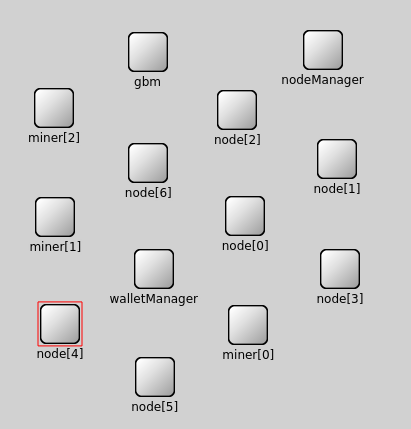
\includegraphics[width=0.5\textwidth]{iblock-qt-network}
	\caption{An \iblock{} network in the OMNeT++'s QT
	environment.}\label{fig:iblock-network}
\end{figure}

Nodes can be of different types, and they can be configured with different
parameters, leveraging the flexibility of the \omnetpp{} framework's
configuration capabilities. In \figref{fig:iblock-network}, two types of nodes
are present: \emph{Miner} nodes and \emph{User} nodes (called just ``node[*]''
in the figure). \emph{Miner} nodes are nodes that contain a \emph{Miner
application} that can mine blocks and earn rewards. \emph{User} nodes are nodes
that have a \emph{TransactionGenerator application} and can send transactions
to the network.

There are other special nodes in the network: The \code{gbm}
(\code{GlobalBlockchainManager}) is responsible of creating the \emph{genesis
block} on startup and removing older blocks from the memory when they are no
longer needed; \code{walletManager} is a node that can be contacted by other
nodes in order to get the address of other nodes' wallets; The
\code{nodeManager} module is used as a directory of all nodes in the network.
Nodes ask the \code{nodeManager} for a reference to another node in the network
when they need to send a message to it. These special nodes will be described
in detail in \secref{sec:impl-global}.

As said before, there are no links between nodes in the network. Instead, nodes
communicate using direct messages sent using the \code{sendDirect()} function
of the \omnetpp{}'s simulation library. Communication between nodes and the
special global nodes is instead done using \emph{Direct Method Calls} (DMCs),
which are an efficient way of calling a method of another module directly,
without the need to send a message.

The choice of using direct messages instead of links was made in order to allow
a fairer comparison of \iblock{}'s performance with other blockchain
simulators, especially with BlockSim \cite{blocksim}, which does not simulate
links between nodes. This choice also simplifies the development of the first
version of the simulator leaving the implementation of a more detailed network
layer for future work.

Each node in the network is a \emph{compound module}. Its internals will be
described in the following sections.

\section{Node model}\label{sec:impl-node}

Bitcoin is a decentralized network of nodes. Thus, the node is the core
component of \iblock{}.

Nodes in \iblock{} are compound modules composed of simple modules that are
called \emph{applications}. Each application is responsible for a specific task
and they all extend the \code{AppBase} class which provides basic
functionalities to applications, allowing for rapid development of new
features.

Nodes are designed to be modular: by selecting the applications that make up a
node, the user can customize the node to have the desired functionality.

As a Bitcoin network state is defined by two main components, the
\emph{blockchain} and the \emph{mempool}, there are two essential applications
in any \iblock{} node: the \code{BlockchainManager} and the
\code{MempoolManager}. All other applications are optional and can be added to
the node as needed using NED language.

Each \iblock{} node has \emph{its own view} of the blockchain and the mempool,
just like in the real Bitcoin network. This means that a node may have a block
that another node does not have, or a transaction that is not in the mempool of
a node may be in the mempool of another node.

\figref{fig:node-internals} shows the internal structure of a miner node that
is also able to generate transactions. All the internal communications between
applications and with the global modules are done using Direct Method Calls
(DMCs), while communication with other nodes is done via messages. The figure
also displays the most important interactions between the applications.

\begin{figure}[tbhp]
	\centering
	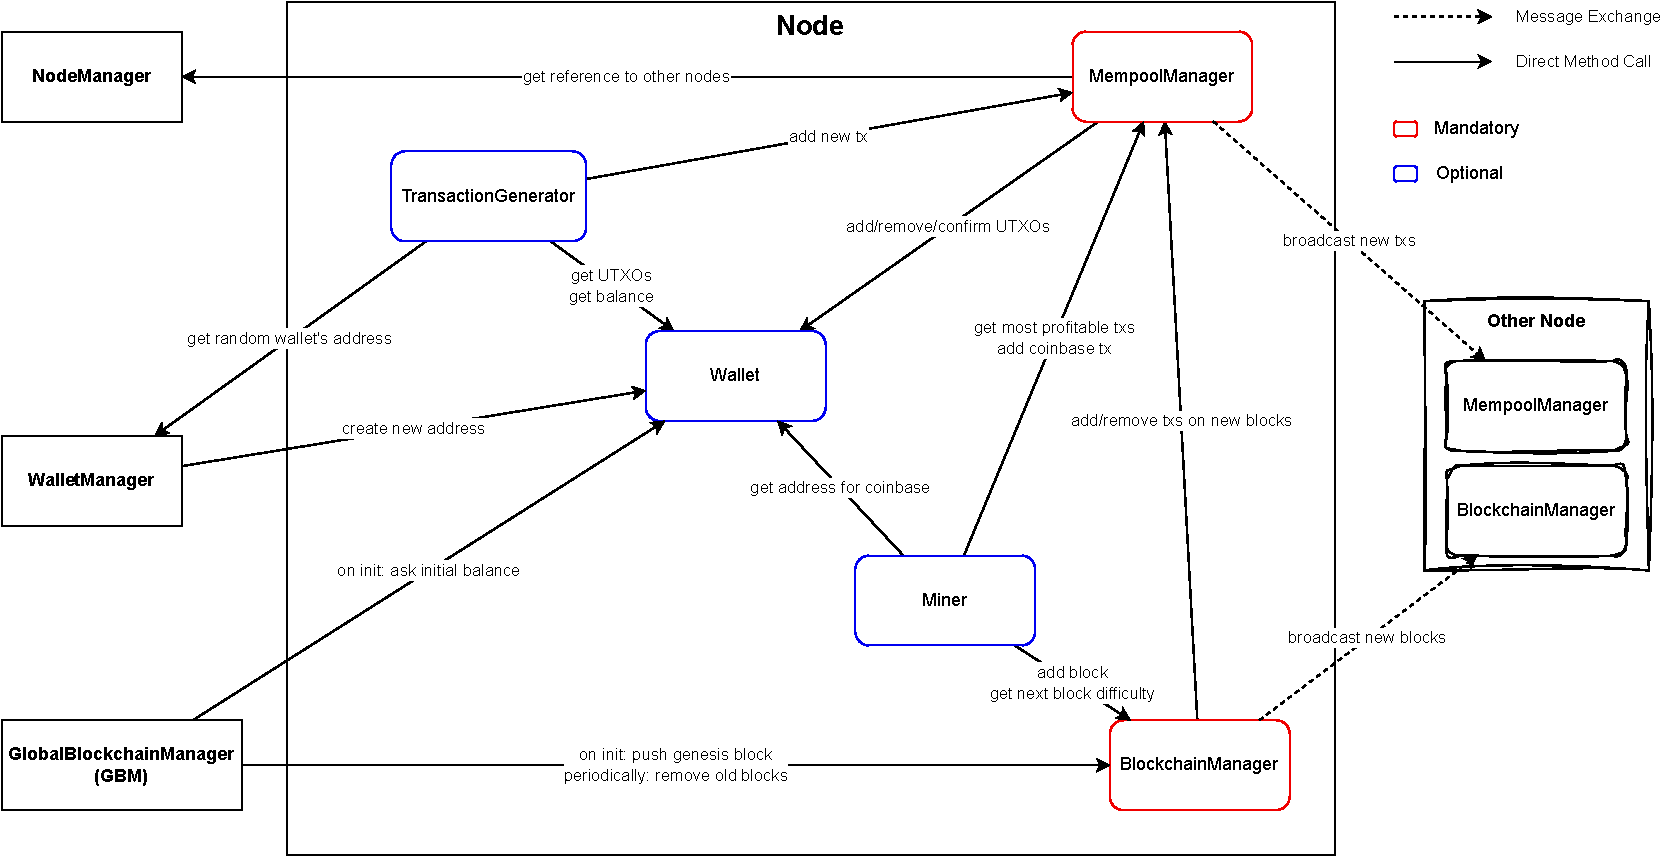
\includegraphics[width=\textwidth]{node-internals}
	\caption{Simple modules (applications) inside a node and the most
	relevant communications between them.}\label{fig:node-internals}
\end{figure}

\subsection{Modular design}\label{subsec:modular-design}

\subsection{Applications}\label{subsec:applications}

This sections describes the applications that are part of a node.
\figref{fig:app-inheritance} shows the inheritance tree of the applications.
The use of the interface \code{IApp} allows to change the implementation of a
specific application only with a configuration change. For example, instead of
the standard \code{BlockchainManager}, a node could use the
\code{SelfishBCManager} described in \secref{sec:selfish-poc} just by inserting
a line in the simulation configuration file:
\begin{verbatim}
Network.node[0].blockchainManager.typename = \
    "iblock.bitcoin.apps.SelfishBCManager"
\end{verbatim}

\begin{figure}[tbhp]
	\centering
	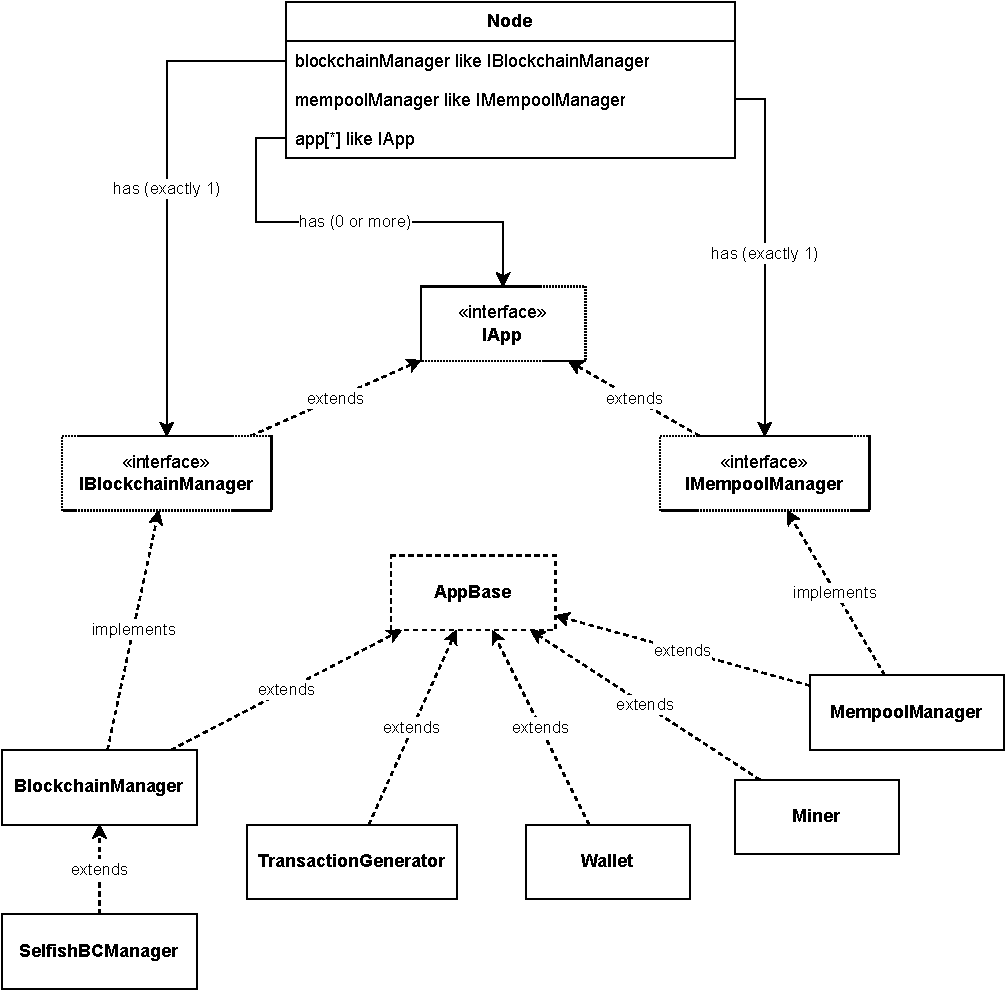
\includegraphics[width=0.8\textwidth]{apps-inheritance}
	\caption{Inheritance tree of the
	applications.}\label{fig:app-inheritance}
\end{figure}

A node can have multiple applications: a miner node, for example, requires a
\code{Miner} application to mine blocks and a \code{Wallet} application to
receive the rewards coming from mining. A node that wants to generate
transactions needs a \code{Wallet} application to store the coins and a
\code{TransactionGenerator} application to generate transactions.

When a message is received from the outside via direct messages (\omnetpp{}'s
\code{sendDirect}), the message is first delivered to the \code{AppBase} class
which in turn calls the \code{handleOtherMessage} method of the application.
The reason behind the name of the method will be discussed later.

The \code{BlockchainManager} and the \code{MempoolManager} applications are
mandatory in any node as they are responsible to maintain the blockchain and
the mempool, respectively.

\subsubsection{BlockchainManager}\label{subsubsec:blockchainmanager}

The \code{BlockchainManager} is responsible for maintaining the blockchain. It
does so by keeping multiple pointer to the head of every branch of the
blockchain. The longest branch is considered the main branch. The developed
application is able to handle forks, chain reorganizations and orphan blocks.

\figref{fig:blockchain-manager-uml} shows the UML diagram of the application.

When a node mines a new block, it broadcasts the block via direct messages to
every other \code{BlockchainManager} in the network. The receiving
\code{BlockchainManager} adds the new block to the blockchain and does the
following:
\begin{enumerate}
	\item If the block is a duplicate block, it is discarded without any
		other side effect;
	\item If the block further extends the main branch it informs the
		\code{MempoolManager} to remove the block's transactions from
		the mempool and the \code{Wallet} application to update the
		number of confirmations associated with each unspent
		transaction output in his possession;
	\item If the block extends a branch that is not the main branch, it
		checks if the branch is longer than the main branch. If so,
		each block in the main branch is removed backward to the
		\emph{fork block} by reinserting the transactions in the
		mempool and unconfirming the UTXOs in the wallet. Then, all
		blocks in the new branch are added to the main branch, one by
		one, by informing the \code{MempoolManager} to remove the
		transactions from the mempool and the \code{Wallet} to confirm
		his UTXOs. If the block is not longer than the main branch, the
		\code{BlockchainManager} just adds the block to the branch;
	\item If the block is an orphan block, it adds it to the array of orphan
		blocks. Orphan blocks are blocks that are received before their
		parent block. When the parent block is received, the orphan
		block is removed from the orphan blocks array and added to the
		blockchain following the same steps as above.
\end{enumerate}

All the above logic is implemented in the \code{appendBlock} method.

At the start of the simulation, the \code{GlobalBlockchainManager} (GBM) module
calls the \code{BlockchainManager}'s \code{addGenesisBlock} to add the genesis
block to the blockchain. The genesis block is a special block which is never
mined in \iblock{}: it is created by the GBM at the start and added to every
\code{BlockchainManager} in the network and it cointains the starting balance
of every \code{Wallet} of the network.

Periodically, the GBM will cal the \code{BlockchainManager}'s \code{cleanup}
method to ask the application to delete the old branches from memory.

When a new block is mined by the local \code{Miner}, it is the responsibility
of the \code{BlockchainManager} to add the block to the blockchain and then
forward the block to the other nodes in the network. This is done by
encapsulating the block in a \code{DirectBlockMsg} message and sending it to
all other nodes via a \code{sendDirect} call. The reference to the other nodes
is obtained from the \code{NodeManager} global module.

Every 2016 blocks, the \code{BlockchainManager} will adjust the difficulty of
the network based on the time needed to mine the last 2016 blocks. This is
implemented in the \code{getNextTargetNBits} method. The difficulty computation
is described in \appendixref{appendix:computations}.

\subsubsection{MempoolManager}\label{subsubsec:mempoolmanager}

The \code{MempoolManager} is responsible for maintaining the mempool. It does
so by a the full list of transactions ordered by their fee rate, thus allowing
an eventual miner to get the list of transactions in the most profitable order.

\figref{fig:mempool-manager-uml} shows the UML diagram of the application.

When a node creates a new transaction, it sends the transaction to every other
\code{MempoolManager} in the network via a direct message. The receiving
\code{MempoolManager} adds the transaction to the mempool and then informs the
wallet if there are new UTxOs that can be spent.

The \code{MempoolManager} class has methods to add and remove transactions from
the mempool. When a transaction is added to the mempool by a local application,
the \code{MempoolManager} contacts the \code{NodeManager} global module to get
the references to all other nodes and then sends the transaction to every other
\code{MempoolManager} by encapsulating it in a \code{DirectTxMsg} message.

\subsubsection{Wallet}\label{subsubsec:wallet}

The \code{Wallet} application is responsible for storing the UTXOs of the node.
Each time the node adds a block to the blockchain or a transaction in the
mempool, the \code{Wallet}'s methods are called to update the list of UTXOs. A
new transaction added to the mempool, causes the \code{MempoolManager} to call
the \code{Wallet}'s \code{addUtxo} method, if the transaction had at least one
output with the \code{Wallet}'s address. When a block is added to the
blockchain, the \code{confirmUtxo} method is used to increase the number of
confirmations of the UTXOs that are still in the wallet. When a transaction
that spends an UTXO is added to the mempool, the \code{removeUtxo} method is
called by the \code{MempoolManager}.

\figref{fig:wallet-uml} shows the UML diagram of the application.

\subsubsection{Miner}\label{subsubsec:miner}

The \code{Miner} application is responsible for mining new blocks. At the start
of the simulation, a \code{nextBlockMsg} timer message is scheduled to be sent
to the \code{Miner} itself. When the message is received, the \code{Miner} will
mine a new block at the top of the current main branch of the blockchain and
inform the \code{BlockchainManager} to add the block to the blockchain (which
will then forward the block to the other nodes in the network). Of course, the
\code{Miner} will also create the coinbase transaction to get the block
reward.

\figref{fig:miner-uml} shows the UML diagram of the application.

Before creating the coinbase transaction, the \code{Miner} asks the
\code{Wallet} application for the address to send the reward. The list of
transactions to include in the block is provided by the \code{MempoolManager}.

The time needed to mine a new block is determined by the \code{Miner}'s hash
rate and the current difficulty of the network. As in the real Bitcoin network,
the difficulty is computed individually by each node and is updated every 2016
blocks by the \code{BlockchainManager}. The computation of the time needed to
mine a block is described in \appendixref{appendix:computations}.

\subsubsection{TransactionGenerator}\label{subsubsec:transactiongenerator}

\section{Blockchain Objects}\label{sec:impl-objects}

In \iblock{}, the two main data structures representing the Bitcoin network
state are the blockchain and the mempool. These are composed of two core object
types: \code{Block} and \code{Transaction} objects.

These objects, along with their composite elements, are defined using
\omnetpp{}'s \emph{message definition} language. This setup allows to
incorporate these objects directly into messages and NED files, enabling them
to be analyzed and modified within the \omnetpp{} QT environment.

Objects in \iblock{} inherit from base classes that include essential
attributes, such as the object hash and size. \figref{fig:objects-uml} presents
the UML diagram of the objects in \iblock{}, with a focus on their base
classes.

\begin{figure}[tbhp]
	\centering
	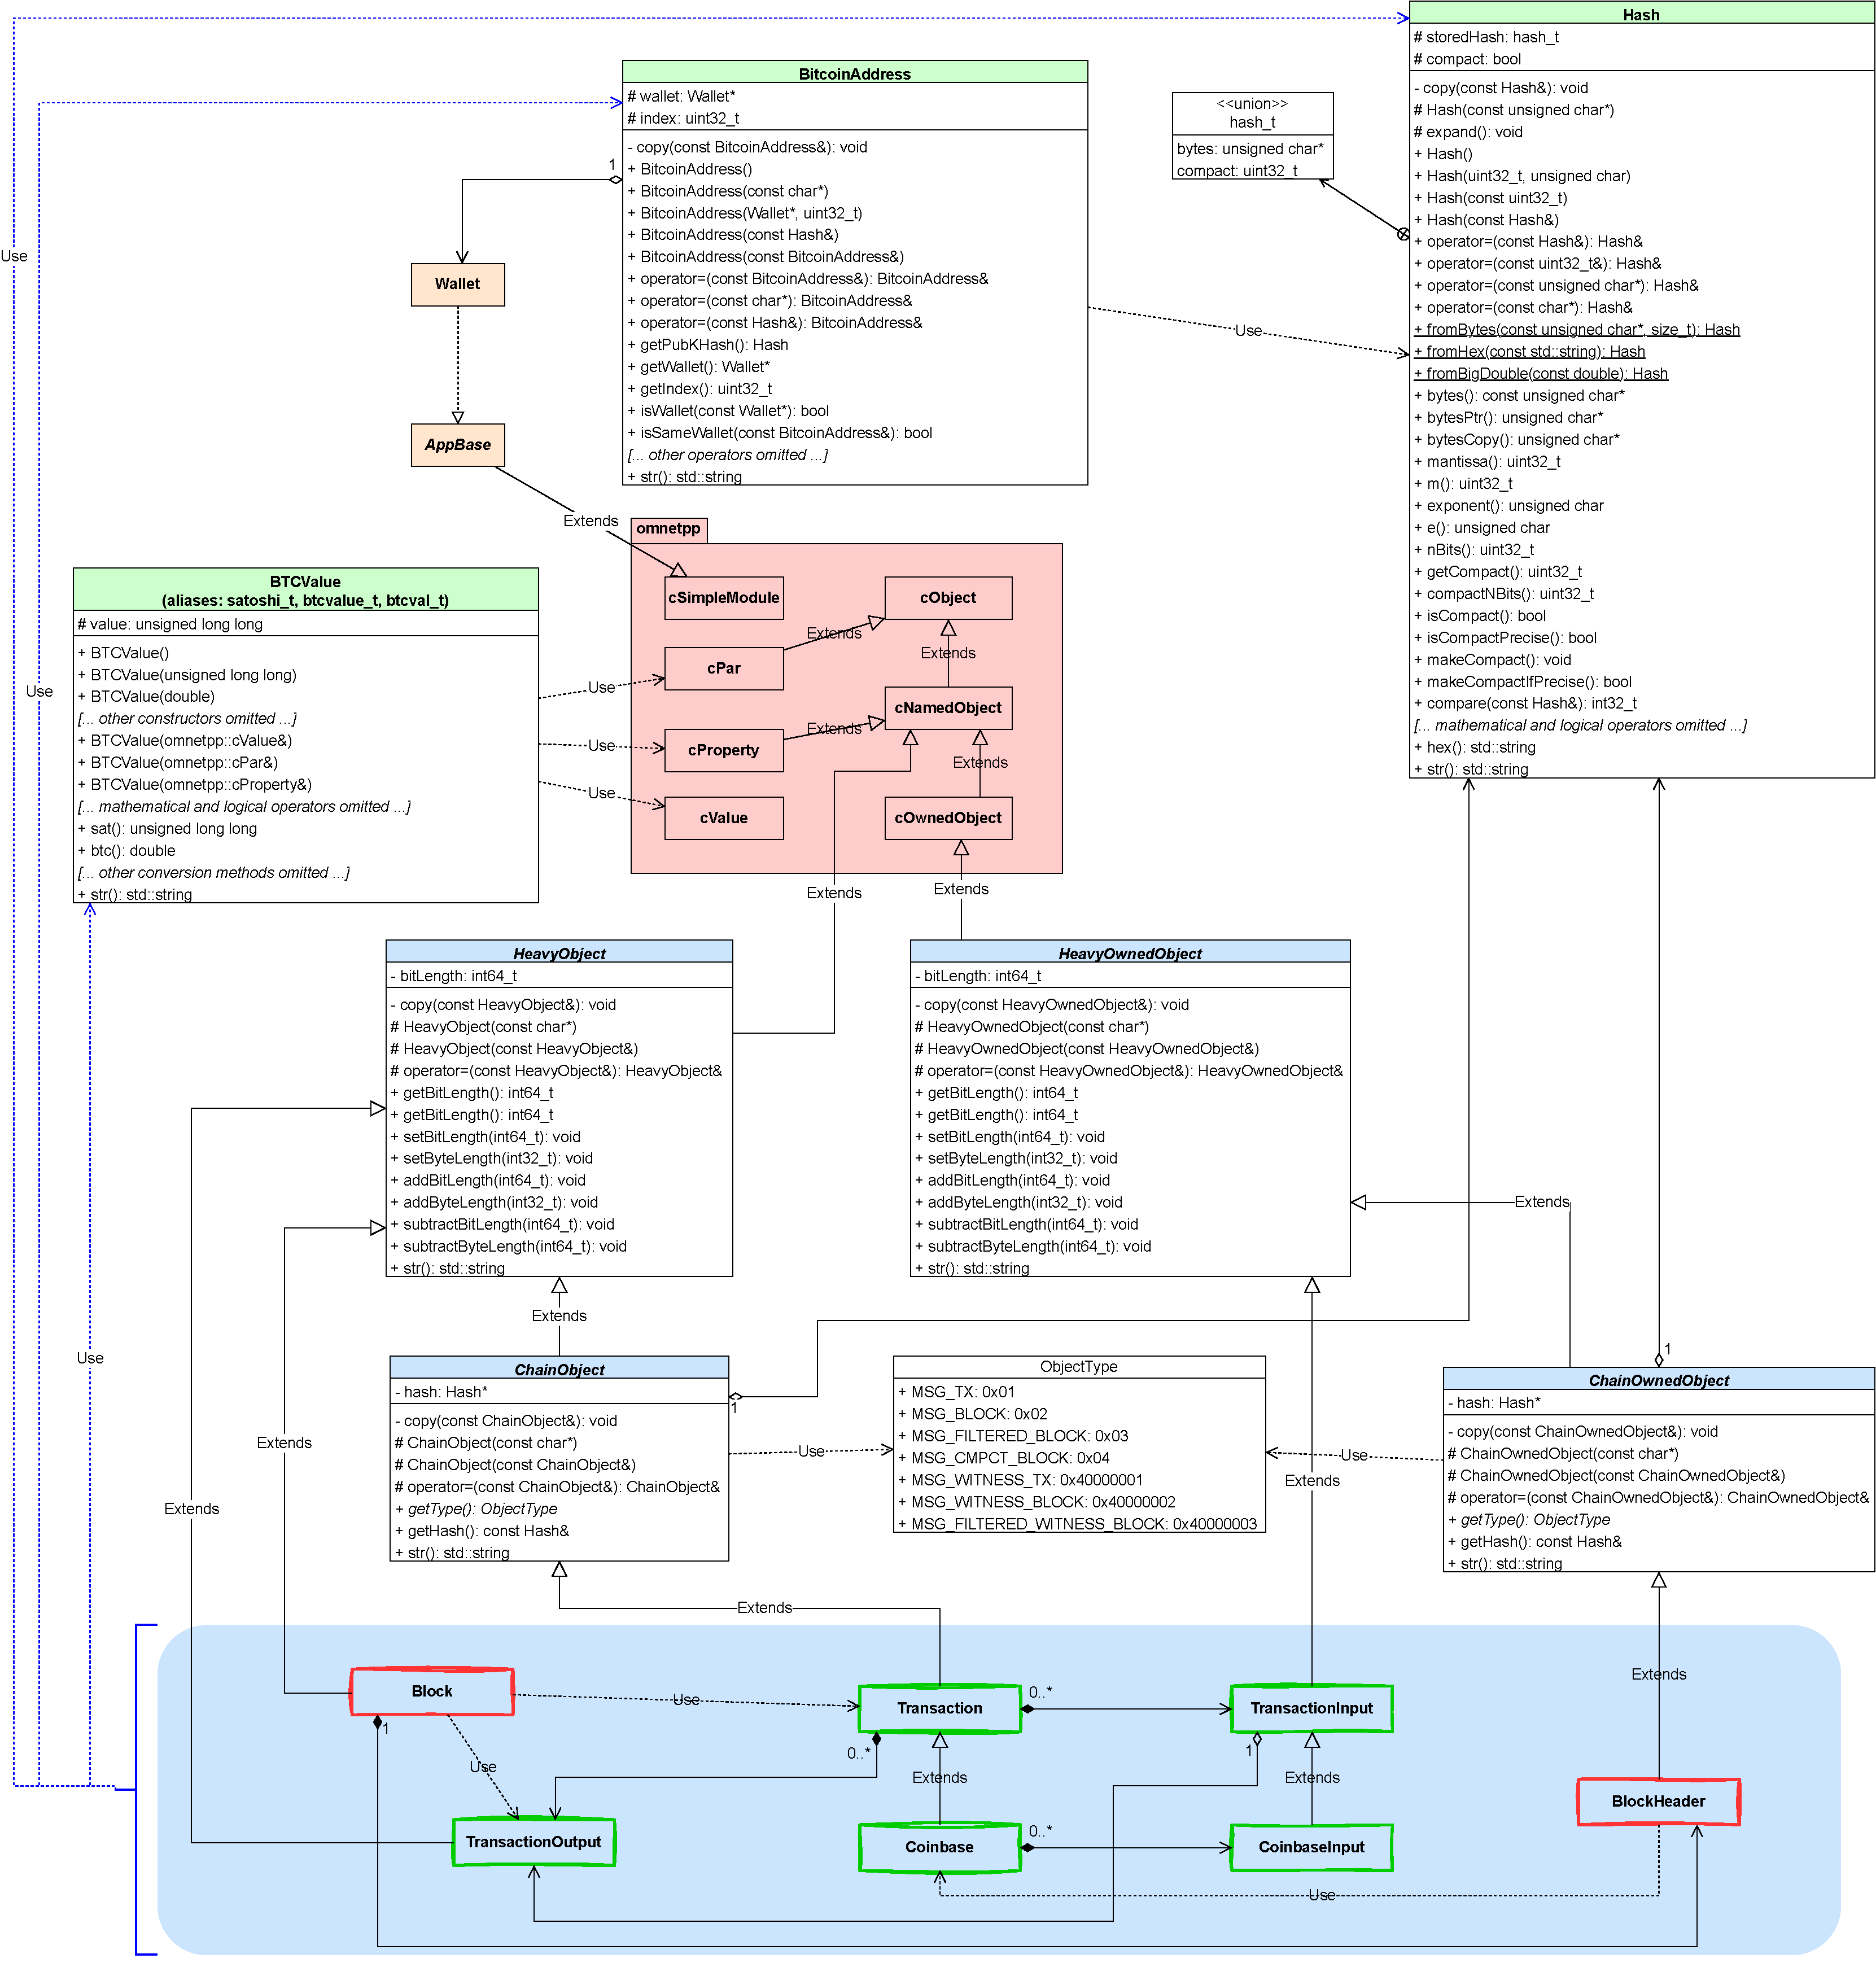
\includegraphics[width=\textwidth]{img/objects-uml}
	\caption{UML diagram of the objects in \iblock{}, highlighting base and
	utility classes. Classes within the blue area represent the core
	objects utilized by the simulation model.}\label{fig:objects-uml}
\end{figure}

\subsection{HeavyObject}\label{subsec:impl-heavyobject}

The \code{HeavyObject} class represents objects with a defined size in bits.
This class inherits from \omnetpp{}'s \code{cNamedObject} class, classifying it
as a \emph{non-owned} object --- meaning no other entity claims ownership of
it. By contrast, the \code{HeavyOwnedObject} class, derived from
\code{cOwnedObject}, is intended for objects with a designated owner.

Ownership in \omnetpp{} supports memory management and sanity checks. When an
object is owned by another, the owner assumes responsibility for its deletion.
Additionally, certain actions, such as sending the object within a message, are
restricted to the owner.

In this structure, the \code{Block} and \code{TransactionOutput} classes extend
\code{HeavyObject}, while the \code{TransactionInput} class derives from
\code{HeavyOwnedObject}. Transaction inputs are always owned by the
\code{Transaction} object they belong to.

\subsection{ChainObject}\label{subsec:impl-chainobject}

The \code{ChainObject} class, derived from \code{HeavyObject}, represents
essential blockchain objects like block headers and transactions. Its
counterpart, \code{ChainOwnedObject}, is derived from \code{HeavyOwnedObject}.

Each \code{ChainObject} has a unique identifier represented by its hash. While
the hash is not actively used in simulation operations, it can be helpful for
debugging and visual inspection within the \omnetpp{}'s QT environment.

Within the class hierarchy, \code{Transaction} is derived from
\code{ChainObject}, while \code{BlockHeader} is derived from
\code{ChainOwnedObject}. Unlike these, the \code{Block} class is based directly
on \code{HeavyObject} rather than \code{ChainObject} --- this is to support
\emph{inventory} messages, which, in the Bitcoin protocol, announce new blocks
using the block header hash rather than the complete block hash. The specific
type of each chain object is defined through the \code{ObjectType} enumeration.

\subsection{Utility Classes}\label{subsec:impl-utility}

There are three utility classes used to support core blockchain functionality
in \iblock{}: \code{Hash}, \code{BitcoinAddress}, and \code{BTCValue}.

\subsubsection{Hash}\label{subsubsec:impl-hash}

The \code{Hash} class enables hash representation, supporting both extended
format (32 bytes) and \emph{compact} format (4 bytes). It is also used to
represent the \emph{target NBits}, the threshold value that a block's hash must
meet to satisfy Proof-of-Work validation.

In Bitcoin and \iblock{}, compact hash format condenses a 256-bit hash into 4
bytes, with the three least significant bytes representing the \emph{mantissa}
and the most significant byte representing the \emph{exponent}. The conversion
from compact to full hash format is shown in \eqref{eq:compact2hash}, where
\(M\) is the mantissa, and \(E\) is the exponent.

\begin{equation}\label{eq:compact2hash}
	H = M \times 256^{(E - 3)}
\end{equation}

Bitcoin treats the mantissa as a signed integer, and \iblock{} adheres to this
convention as well \cite{bitcoin-dev}. If the mantissa is negative, the compact
representation can be adjusted by dividing the mantissa by 256 and increasing
the exponent by one, which yields an equivalent value with a different
encoding. The \code{Hash} class performs this adjustment automatically.

\subsubsection{BitcoinAddress}\label{subsubsec:impl-bitcoinaddress}

In \iblock{}, Bitcoin addresses are represented by a pointer to the owning
\code{Wallet} module and an integer index, allowing each \code{Wallet} to hold
multiple addresses. The \code{BitcoinAddress} class also provides methods to
retrieve a hash that uniquely represents the address.

\subsubsection{BTCValue}\label{subsubsec:impl-btcvalue}

The \code{BTCValue} class enables configuration and NED files to represent
Bitcoin amounts in various units, such as BTC (Bitcoins), mBTC
(milli-bitcoins), and satoshis (\(10^{-8}\) BTC). Internally, values are stored
in satoshis, Bitcoin's smallest unit. The class includes multiple \emph{getter}
methods for retrieving amounts in different units.

This class also facilitates extraction of values from NED parameters and
properties by directly assigning the parameter or property to a \code{BTCValue}
object. Additionally, it supports a wide range of mathematical and logical
operations.

\subsection{Modeling Transactions}\label{subsec:impl-transactions}

In \iblock{}, transactions are represented by the \code{Transaction} class. The
structure and composition of this class are illustrated in
\figref{fig:transaction-uml}.

\begin{figure}[tbhp]
	\centering
	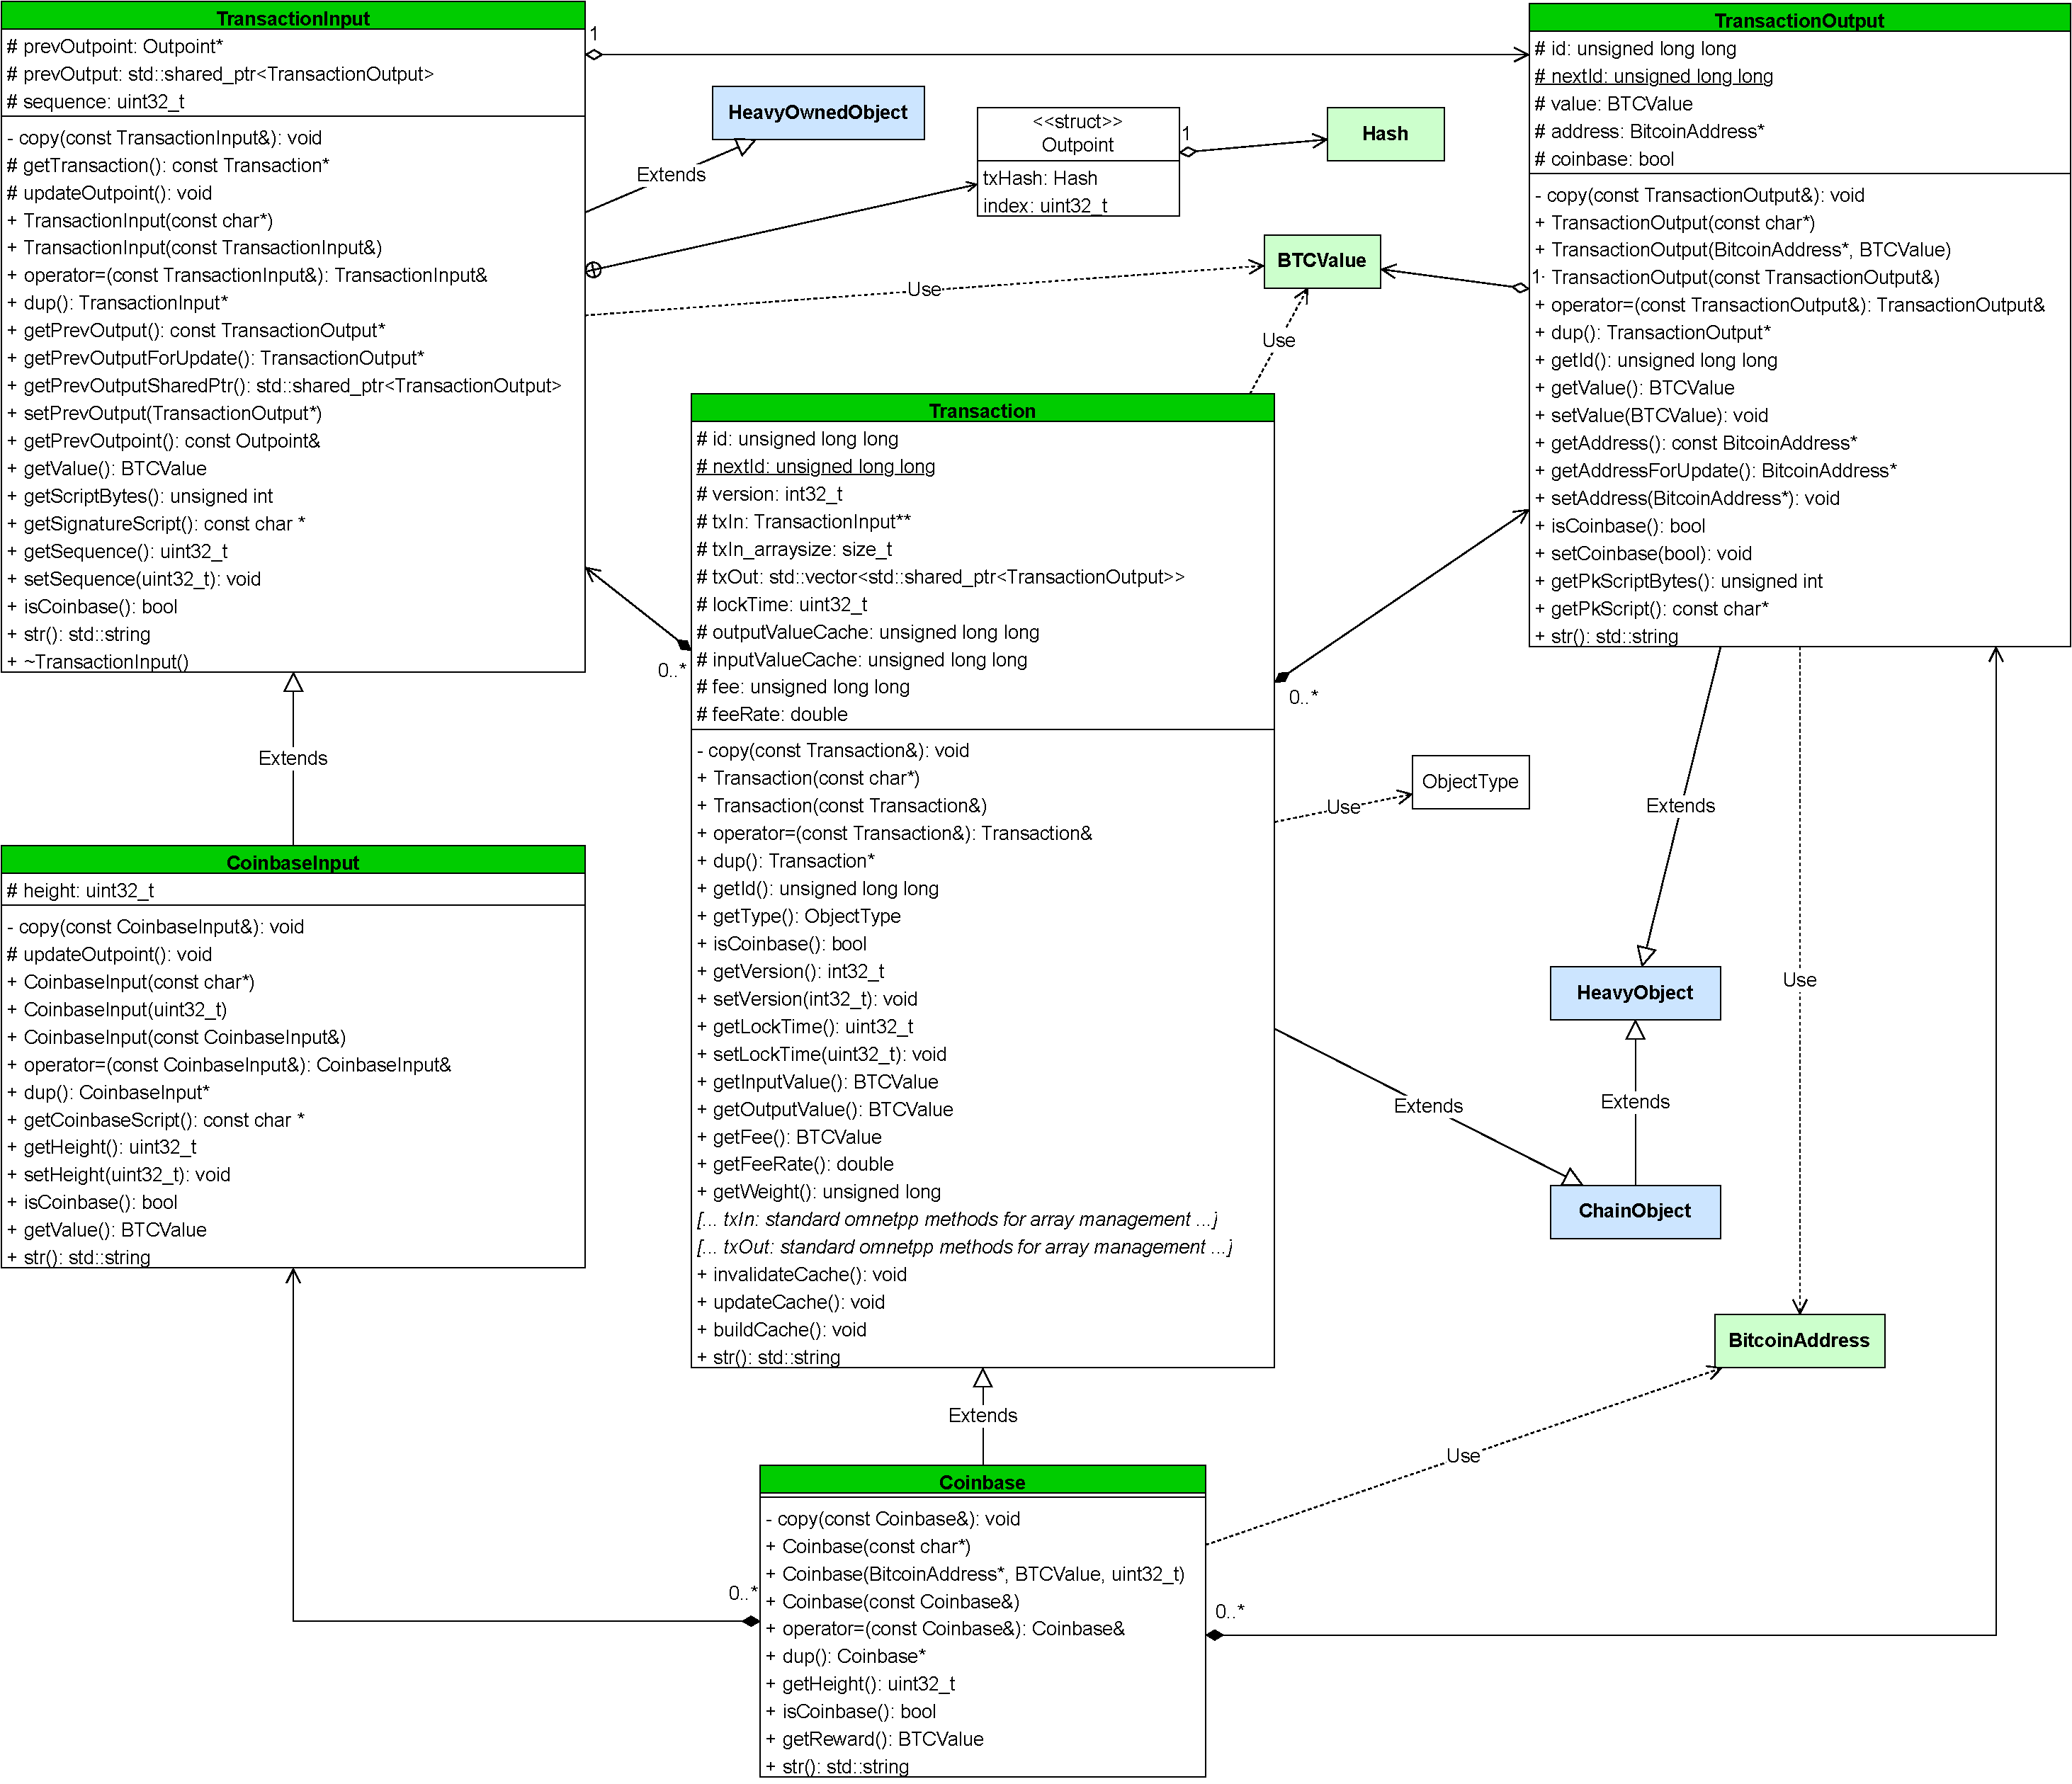
\includegraphics[width=\textwidth]{img/transaction-uml}
	\caption{UML diagram of the \code{Transaction} class and its component
	classes.}\label{fig:transaction-uml}
\end{figure}

Following the Bitcoin protocol, each \code{Transaction} consists of multiple
inputs (\code{TransactionInput}) and outputs (\code{TransactionOutput}). Each
\code{TransactionInput} refers to a specific \code{TransactionOutput} from a
prior transaction.

The \code{Coinbase} class extends \code{Transaction} to represent a coinbase
transaction, which is used to reward miners. This transaction includes a single
special input, \code{CoinbaseInput}, which does not reference any previous
output.

\iblock{} transactions incorporate all fields supported by the Bitcoin
protocol. Additionally, certain fields in the \code{Transaction} class act as a
\emph{cache}, storing values computed from other fields. These optimizations
are covered in \secref{sec:optimizations}.

Memory management is handled with \emph{smart pointers} to maintain efficient
references. For instance, references to transaction outputs are stored as smart
pointers, as they are shared across different components: each \code{Wallet}
maintains a list of unspent transaction outputs (instances of
\code{TransactionOutput}), each transaction input references a prior output,
and UTXO lists are also stored within the \code{Block} object for performance
reasons.

\subsection{Modeling Blocks and the Blockchain}\label{subsec:impl-blocks}

\figref{fig:block-uml} presents the UML diagram of the \code{Block} and
\code{BlockHeader} classes. Each \code{Block} contains a \code{BlockHeader} and
a list of transactions. The fields in \code{BlockHeader} mirror those in an
actual Bitcoin block header.

\begin{figure}[tbhp]
	\centering
	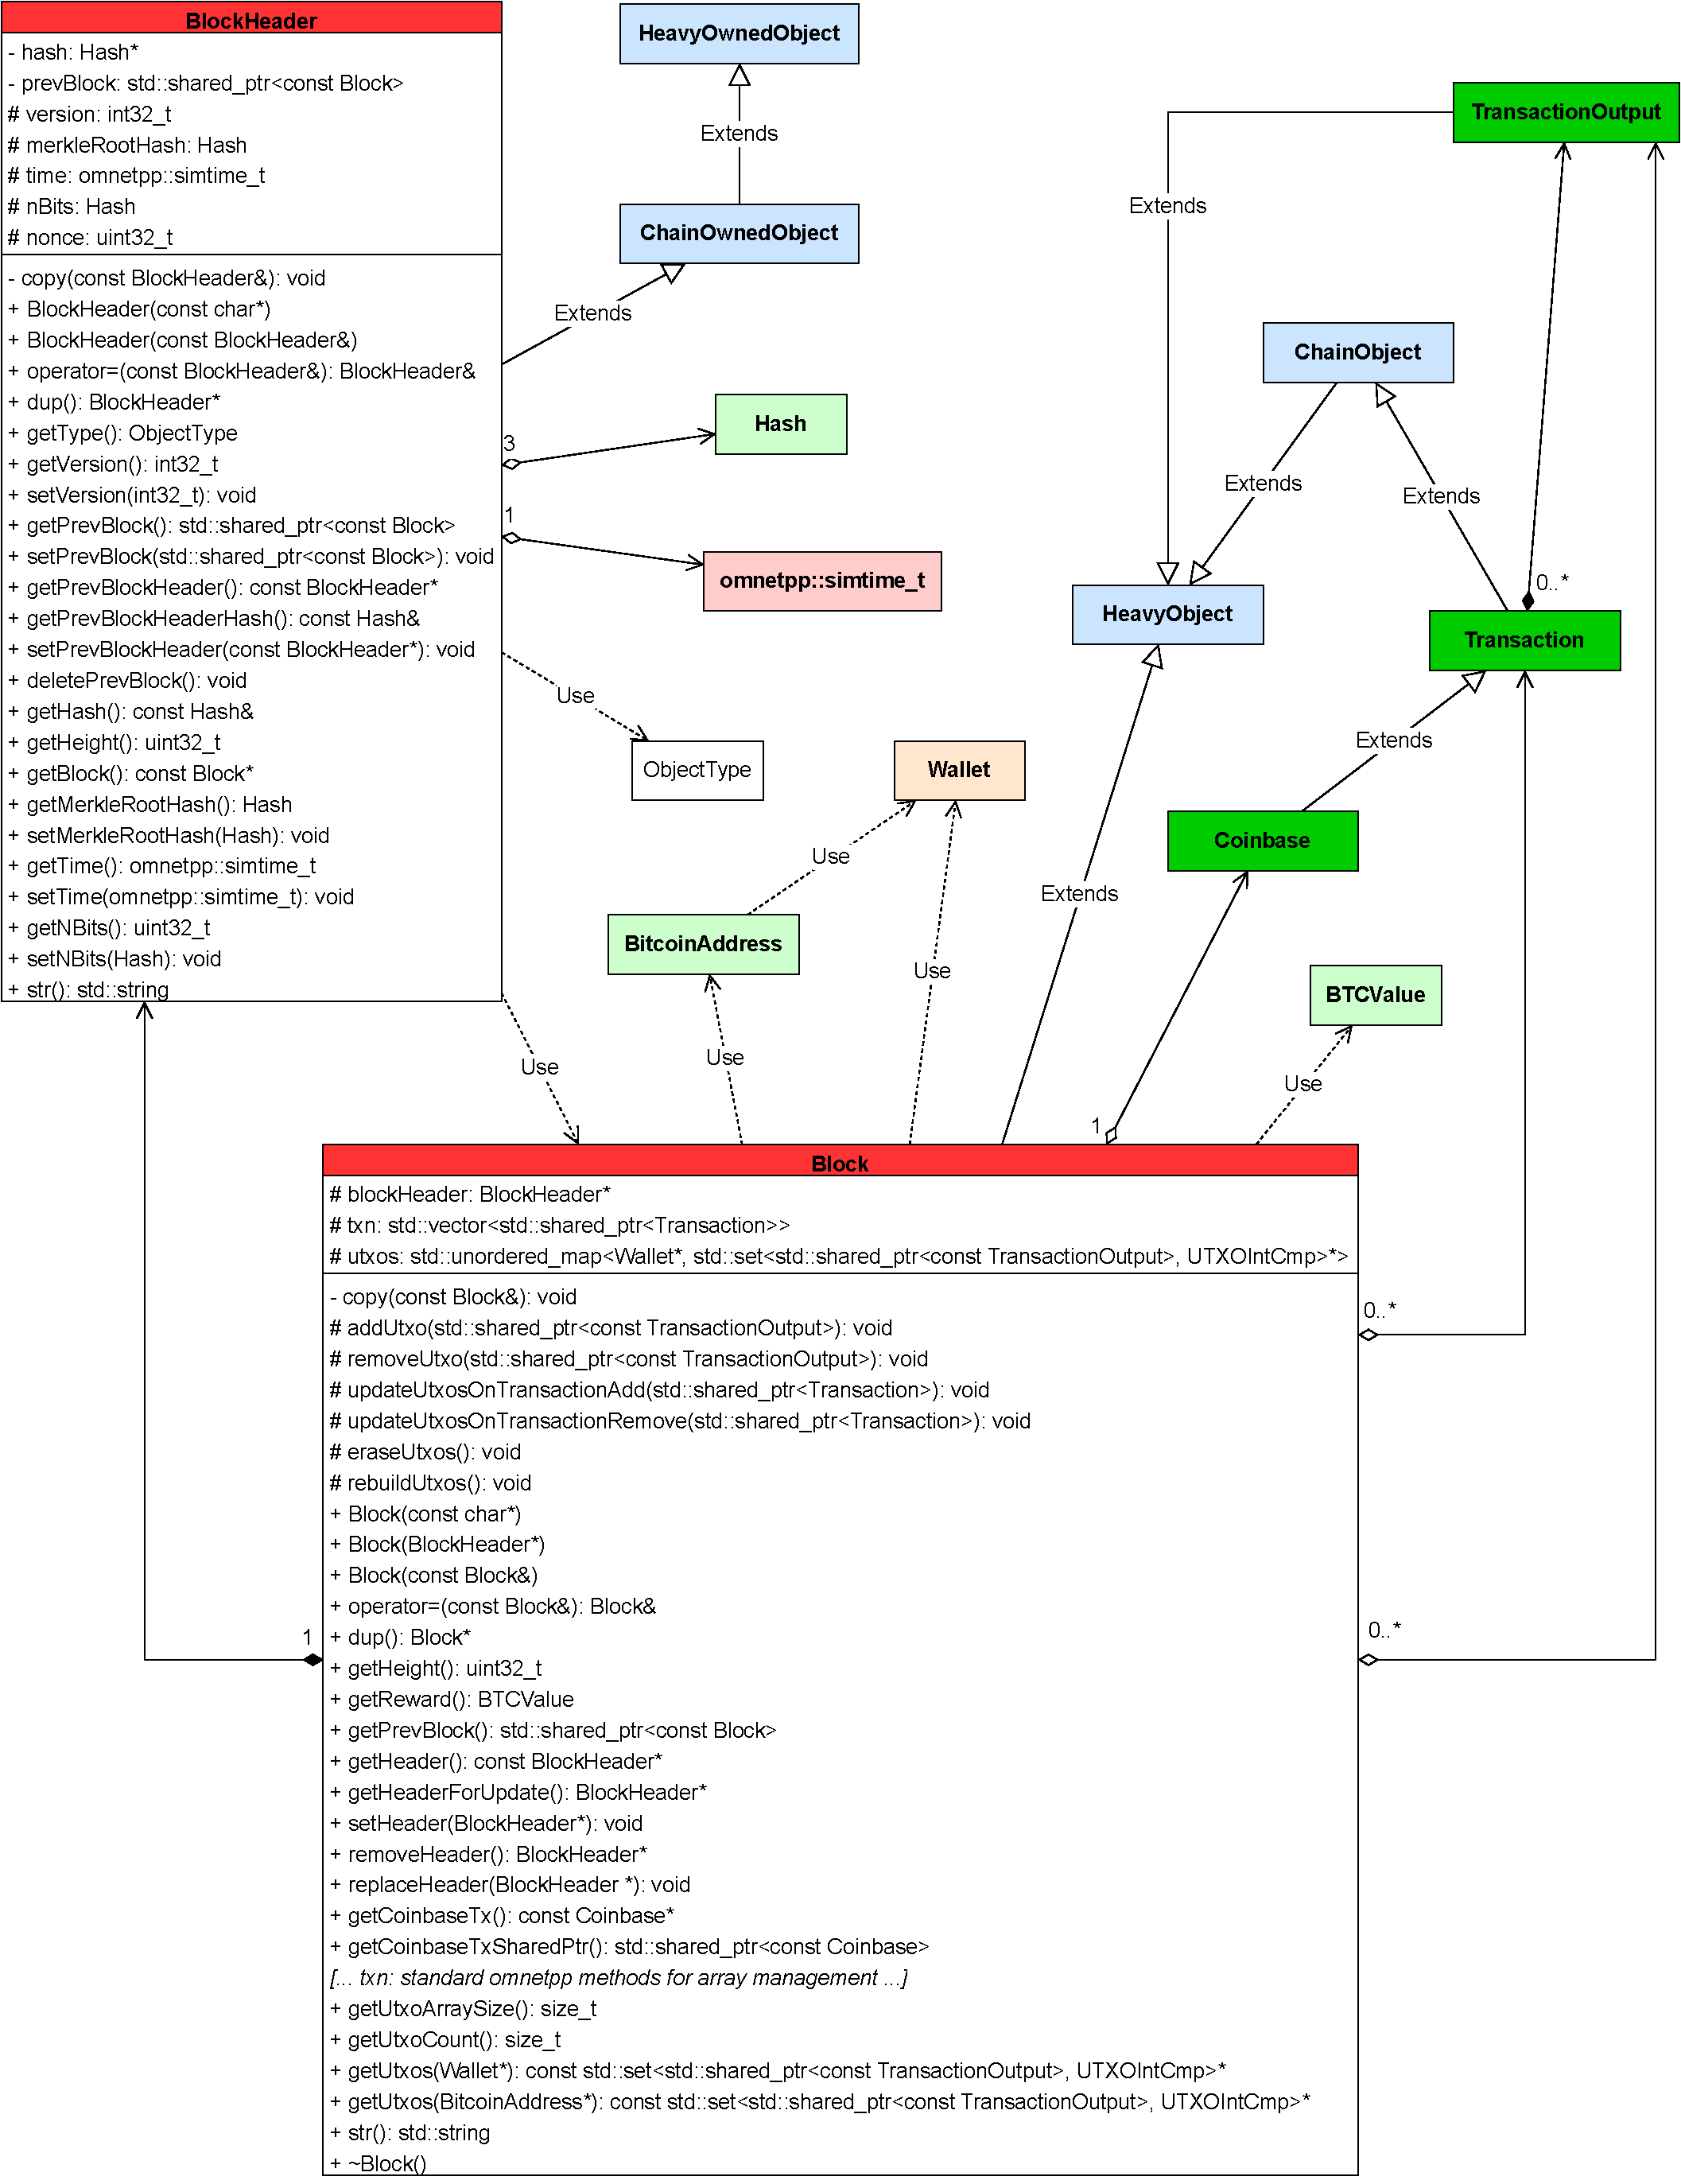
\includegraphics[width=\textwidth]{img/block-uml}
	\caption{UML diagram of the \code{Block} and \code{BlockHeader}
	classes.}\label{fig:block-uml}
\end{figure}

The \code{Block} class maintains an updated list of UTXOs (Unspent Transaction
Outputs), which is built as transactions are added to the block. This process
takes UTXOs from the previous block, removes spent outputs, and adds new ones
from current transactions. Nodes rely on this list to retrieve UTXOs for their
wallets, combining them with UTXOs from the mempool.

Blocks are linked through smart pointers held in their headers, which enables
the \code{GBM} (Global Blockchain Manager) to remove obsolete blocks from
memory efficiently. Transactions are also referenced by smart pointers,
ensuring that if a block is deleted, its transactions are also removed ---
unless referenced elsewhere, such as by other blocks or a node's mempool.

\section{Global Modules}\label{sec:impl-global}

In \figref{fig:app-uml} on page \pageref{fig:app-uml}, the green-highlighted
classes represent the global modules within the simulation. These modules,
external to individual nodes, provide essential services across the network.

Global modules identify nodes and applications in the network through
\omnetpp{}'s topology discovery and NED properties. For example, each network
node has a \code{@bitcoinNode} property, each wallet is tagged with
\code{@wallet}, and each \code{BlockchainManager} is marked with
\code{@blockchainManager} in their NED definitions.

The \code{NodeManager} module serves as a directory of all nodes, maintaining
an array of them accessible via the \code{nodes()} method, which allows for
node iteration in loops. This module is used by \code{BlockchainManager} and
\code{MempoolManager} for block and transaction propagation across the network.

The \code{WalletManager} module supports the \code{TransactionGenerator}
application by supplying new Bitcoin addresses (instances of the
\code{BitcoinAddress} class) for random wallets throughout the network.

The \code{GBM} module is slightly more complex and it is described in the
following section.

\subsection{The Global Blockchain Manager}\label{subsec:impl-global-gbm}

The \code{GBM} (Global Blockchain Manager) module is responsible for creating
the \emph{genesis block} and managing memory by cleaning out obsolete blocks.

In a Bitcoin network, the genesis block is the initial block in the blockchain.
Unlike regular blocks, it lacks standard transactions since there's no
pre-existing Bitcoin in circulation; only the coinbase transaction generates
the first coins. In the Bitcoin protocol, this coinbase transaction typically
contains 50 bitcoins, but in \iblock{}, the genesis block's coin amount can be
adjusted. Additionally, these initial funds can be distributed across multiple
wallets in the network based on user-defined starting balances.

When setting up the simulation, the user specifies each wallet's initial
balance in the simulation configuration. The \code{GBM} then assigns these
amounts within a single coinbase transaction in the genesis block, with each
output directed to a designated wallet. The \code{GBM} then distributes the
genesis block to all \code{BlockchainManager} instances in the network using
the \code{addGenesisBlock()} method. In this way, when the simulation starts,
each wallet will have its initial balance given by the genesis block.

Once the genesis block is established in all network blockchains, the
simulation begins. The \code{GBM} module periodically wakes to perform memory
cleanup, freeing space from blocks (and transactions) that are no longer
necessary.

The cleanup process is as follows:
\begin{enumerate}
	\item Each time a \code{BlockchainManager} adds a new block to its main
		blockchain branch, it notifies the \code{GBM}. The \code{GBM}
		stores a reference to this block in a map tracking all main
		branches across the network;
	\item On each \code{GBM} wake (configurable interval), it identifies
		the common ancestor of all main branches. The \code{GBM} then
		retains this common ancestor and its parent, discarding all
		older blocks. Deletion is managed by removing the parent
		pointer from the earliest retained block. Thanks to smart
		pointers, all blocks without remaining references are
		automatically deleted;
	\item The \code{GBM} then calls each \code{BlockchainManager}'s
		\code{cleanup()} method, passing the height of the retained
		common ancestor. Each \code{BlockchainManager} then removes any
		branches whose head height is below this threshold.
\end{enumerate}

By using smart pointers, blocks are deleted simply by removing references, and
transactions within blocks are also automatically removed once they are no
longer referenced by any block or any mempool.

The \code{GBM} module has a single configurable parameter:
\code{cleanupInterval}, which defines the time between memory cleanup
operations. By default, this interval is set to one hour (simulated time).

This memory management approach allows \iblock{} to handle large-scale
simulations efficiently, maintaining essential blocks and transactions without
memory overflow. If an applications must ensure that a block or a transaction
is retained in memory, it just need to keep a reference to it.

\section{Collected Statistics}\label{sec:statistics}

During simulation, \iblock{} collects a range of statistics using \omnetpp{}'s
signal mechanism. In this approach, simulation modules emit signals, which
\omnetpp{} collects according to the NED file specifications.

Most statistics are gathered on a per-node basis, reflecting the decentralized
nature of a Bitcoin network. This structure means that the number of potential
statistics grows linearly with the number of nodes, though users can configure
simulations to focus only on specific statistics of interest.

Statistics can be collected as time series (vectors), aggregated values
(scalars), or histograms, depending on the needs of the analysis.

Table~\ref{tab:network-statistics} provides an overview of network-level
statistics tracked by \iblock{}, while Table~\ref{tab:node-statistics} on
page~\pageref{tab:node-statistics} details the node-level statistics collected.

\begin{table}[tbhp]
	\tiny
	\centering
	\begin{tabularx}{\linewidth}{|r|c|c|X|}
		\toprule
		Name & Unit & Recorders\footnotemark & Description \\
		\midrule
		\code{blocks} & int & vector, count, timeavg & Total number of
		blocks mined.\\\midrule
		\code{circulatingSupply} & satoshis & vector, stats, last &
		Quantity of Bitcoins circulating in the entire
		network.\\\midrule
		\code{fees} & satoshis & vector, stats, last & Total fees paid
		by nodes to create transactions.\\\midrule
		\code{processedTransactions} & int & vector, stats, sum,
		histogram & Total number of transactions included in
		blocks.\\\midrule
		\code{transactions} & int & vector, stats, last & Total number
		of transactions created. \\\midrule
		\code{walletAddresses} & int & vector, last & Total number of
		Bitcoin addresses created.\\
		\bottomrule
	\end{tabularx}
	\caption{Network-level statistics
	collected.}\label{tab:network-statistics}
\end{table}
\footnotetext{See the \citetitle{omnetpp-simulation-manual} for the meaning of
statistics filters and recorders reported in this column
\cite{omnetpp-simulation-manual}.}

\begin{table}[tbhp]
	\tiny
	\centering
	\begin{tabularx}{\linewidth}{|c|r|c|c|X|}
		\toprule
		Application & Name & Unit & Recorders & Description \\\midrule
		\code{BlockchainManager} & \code{duplicateBlocks} & int &
		vector, count & Number of duplicate blocks received.\\\midrule
		\code{BlockchainManager} & \code{forks} & int & vector(sum),
		count & Number of side branches created.\\\midrule
		\code{BlockchainManager} & \code{mainBranchLength} & int &
		vector, stats, last & Height of the blockchain's main
		branch.\\\midrule
		\code{BlockchainManager} & \code{mainBranchSwaps} & int &
		vector, count & Number of chain reorganizations
		performed.\\\midrule
		\code{BlockchainManager} & \code{mainBranchTransactions} & int
		& vector(sum), histogram, last(sum) & Number of transactions
		included in the blockchain's main branch.\\\midrule
		\code{BlockchainManager} & \code{networkDifficulty} & double &
		vector, stats, last & Current mining difficulty of the
		network.\\\midrule
		\code{BlockchainManager} & \code{orphans} & int & vector &
		Number of orphan blocks stored with the blockchain.\\\midrule
		\code{MempoolManager} & \code{mempoolSize} & bytes & vector,
		stats, last & Size of the mempool, in bytes.\\\midrule
		\code{MempoolManager} & \code{transactionCount} & int & vector,
		stats, max, last & Number of transactions in the
		mempool.\\\midrule
		\code{Miner} & \code{blockMined} & int & vector, count, timeavg
		& Number of blocks found by the miner.\\\midrule
		\code{Miner} & \code{blockReward} & satoshis & vector,
		histogram, stats, sum & Revenues from blocks mined, including
		revenues that does not have reached \code{coinbaseMaturity} and
		those from blocks added to side branches.\\\midrule
		\code{Miner} & \code{blockRewardPerByte} & satoshis/byte &
		vector, histogram, stats & Simply
		\code{blockReward}/\code{blockSize}.\\\midrule
		\code{Miner} & \code{blockSize} & bytes & vector, histogram,
		stats, sum & Size of each block mined.\\\midrule
		\code{Miner} & \code{blockTime} & time & vector, histogram,
		stats & Time spent mining each block.\\\midrule
		\code{Miner} & \code{transactionsProcessed} & int & vector,
		histogram, stats, sum & Number of transaction processed by the
		miner \idest{added to mined blocks}.\\\midrule
		\code{TransactionGenerator} & \code{createdTransactions} & int
		& vector, stats, last & Number of transactions
		created.\\\midrule
		\code{TransactionGenerator} & \code{transactionFee} & satoshis
		& vector, histogram, sum & Paid fees for each
		transaction.\\\midrule
		\code{TransactionGenerator} & \code{transactionFeeRate} &
		satoshis/byte & vector, histogram & Fee rate for each
		transaction created. \\\midrule
		\code{TransactionGenerator} & \code{transactionInputCount} &
		int & vector, histogram & Number of inputs in each transaction
		created.\\\midrule
		\code{TransactionGenerator} & \code{transactionInputValue} &
		satoshis & vector, histogram, sum & Total value of inputs in
		each transaction.\\\midrule
		\code{TransactionGenerator} & \code{transactionOutputCount} &
		int & vector, histogram & Number of outputs in each transaction
		created.\\\midrule
		\code{TransactionGenerator} & \code{transactionOutputValue} &
		satoshis & vector, histogram, sum & Total value of outputs in
		each transaction.\\\midrule
		\code{TransactionGenerator} & \code{transactionSize} & bytes &
		vector, histogram, sum & Size of each transaction
		created.\\\midrule
		\code{Wallet} & \code{createdAddresses} & int & vector, last &
		Number of addresses created by the wallet.\\\midrule
		\code{Wallet} & \code{miningEarnings} & satoshis & vector,
		histogram, last & Mining revenues, including block subsidies
		and fees, counted only when \code{coinbaseMaturity} is reached
		by the coinbase transaction.\\\midrule
		\code{Wallet} & \code{utxoCount} & int & vector, stats, max,
		last & Number of UTXOs in the wallet.\\\midrule
		\code{Wallet} & \code{utxoDuration} & int (blocks) & vector,
		stats, histogram & Time difference between the insertion of a
		new UTXO in the wallet and when it is spent, measured in
		blocks.\\\midrule
		\code{Wallet} & \code{walletBalance} & satoshis & vector,
		stats, max, last & Amount of Bitcoins in wallet.\\
		\bottomrule
	\end{tabularx}
	\caption{Node-level statistics collected.}\label{tab:node-statistics}
\end{table}

